\chapter{Vectors: How far and which direction to the nearest pub?}
\epigraph{ ``[The vector] has never been of the slightest use to any creature.''}
{{\normalfont ---\ Lord Kelvin}}

\label{apx:vectors}

\section{Magnitude and Direction}
If I were to ask you, ``How hot is it today?'' You would respond with a single
number for the temperature.  If I were to ask, ``Where is the nearest pub?'' You
would likely tell me both how far and what direction to walk.

Why would you respond to the former question with one value while giving two
values for the latter?

Some physical quantities such as temperature, mass, charge, and energy require
one value in space and time to completely describe them.  Others such as
velocity, gravitational acceleration, electric field strength, and heat flow are
directional and require both a magnitude and direction to fully describe them.
So lets explore the world of vectors as we will encounter many in the course of
study.

Returning to the question of the nearest pub, you might tell me that there is
one three blocks south and four blocks west.  You gave me both a direction to
walk and a distance to travel.  But you did more than that.  Since the streets
of Adelaide proper are laid out on a north--south and east-west grid you
provided be with directions I would have to walk to get there (the
components).  So we can write down my position vector relative to the
pub mathematically as
\begin{equation}
    \vb{r} = (r_x,r_y) ,
\end{equation}
where $\vb{r}$ is the position vector and $r_x$ and $r_y$ are my distances north
and east of the pub.  The For the sake of simplicity we need to make a couple
assumptions:
\begin{itemize}
    \item the distance of a north-south block is the same as the distance of an
    east-west block (i.e. unit distances in the $x$, and $y$ directions are
    equivalent length); and
    \item north-south and east-west blocks are at right angles (i.e. the axes
    are {\it orthogonal} to each other).
\end{itemize}
These assumptions will simplify the math and are standard for any Cartesian
reference frame.  However, axes need not be orthogonal as we see for hexagonal
and triclinic mineral systems but we won't use these in the course.
\begin{figure}[hbt]
    \centering
    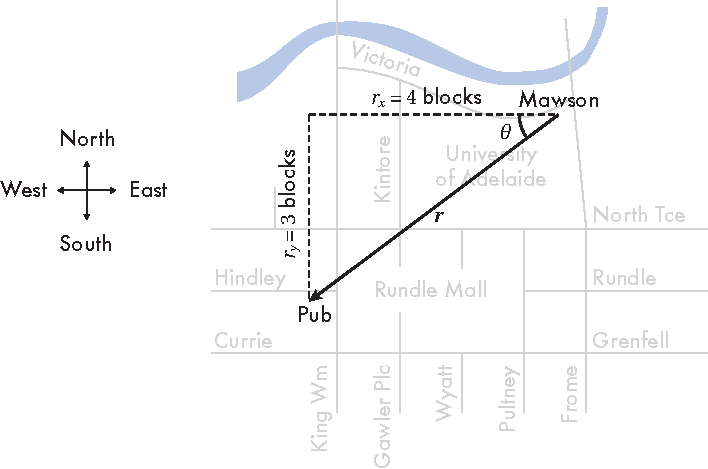
\includegraphics[]{math_primer/figures/position_vector.pdf}
    \caption{Position vector from Mawson Labs to a nearby pub.}
    \label{fig:posvec}
\end{figure}

\ntextbox{Notation}{
    When discussing vectors we use a bold letter, e.g, $\vb{r}$.  Since it is difficult to bold characters on a chalkboard or paper there are some common notations for vectors: $\vec{r}$ or $\utilde{r}$.  Likewise, there are multiple ways to write the components of a vector.  The components are frequently written with a subscript indicating the direction to which they refer, e.g. $r_x$.  As above, we can represent a vector as $\vb{r} = (r_x,r_y)$.  We can also write a vector in terms of it's components as
    \[
        \vb{r} = r_x \vu{x} + r_y \vu{y} ,
    \]
    where $\vu{x}$ and $\vu{y}$ are unit vectors, vectors of unit length in the direction of the labeled axis.  Because the direction of the unit vectors are orthogonal they cannot be added to produce a single quantity.
}{alert}

The directions to the pub are the vector components, but what I am interested in are the distance and direction from Mawson Labs.  We need a way to compute the distance from the components.  But we cannot simply add the length of $r_x$ and the length of $r_y$ because they are in mutually exclusive directions.  As you can see in Figure~\ref{fig:posvec} the individual components form the legs of a right triangle with the hypotenuse defined as the position vector.  So all we have to do is remember the Pythagorean theorem.  We can then write the magnitude/length/norm of the position vector as
\begin{equation}
    \norm{\vb{r}} = r = (r_x^2 + r_y^2)^{1/2} ,
\end{equation}
where $\norm{r}$ is called the norm.  Since we are lazy, we typically just write the magnitude as a roman, rather than bold, $r$.  Note: the norm is always positive.

The direction is determined by the signed ratio of the components
\begin{equation}
    \theta = \tan^{-1} \left( \frac{r_y}{r_x} \right),
\end{equation}
where $\tan^{-1}$ is the inverse of the tangent function.  Since the tangent
function has a $90\deg$ ambiguity, defined from $[-\pi/2,\pi/2]$ radians, we
must keep track of the sign on the $x$-component and add an additional $\pi$
radians if $r_x$ is negative.

We can extend our definitions to 3-dimensional space (suppose I had to go down
some stairs to get to the pub) by
\begin{equation}
    \norm{\vb{r}} = (r_x^2 + r_y^2 + r_z^2)^{1/2} .
\end{equation}
The direction is a bit trickier in this case since I now need two angles to
describe the orientation of my position vector.  We can define one angle as
before, but the second is defined as
\begin{equation}
    \phi = \cos^{-1} \left( \frac{r_z}{r} \right).
\end{equation}


\section{Changing of coordinate systems}
We will now consider several properties of a vector before turning to the rules .

\section{Addition and subtraction}

Adding vectors is very simple.  Graphically, we can add vectors by placing the
tail of one on the head of another (Figure~\ref{fig:sumdiff}.  The resultant
vector is determined simply by separately summing the individual components,
\begin{equation}
    \vb{a} + \vb{b} = (a_x + b_x)\vu{x} 
    + (a_y + b_y)\vu{y} + (a_z + b_z)\vu{z} .
\end{equation}
\begin{figure}[hbt]
    \centering
    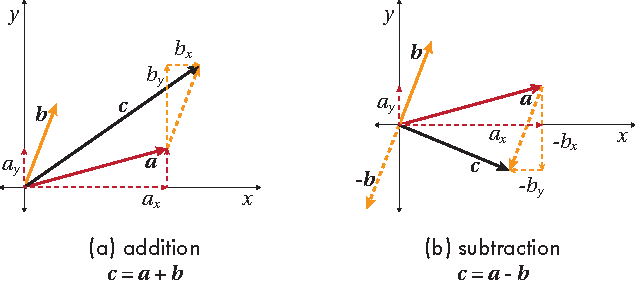
\includegraphics[]{math_primer/figures/vectors_sumdiff.pdf}
    \caption{Vector addition (a) and subtraction (b) in two dimensions.}
    \label{fig:sumdiff}
\end{figure}

Subtraction of vectors is very similar to the addition, again minding the
individual components,
\begin{equation}
    \vb{a} - \vb{b} = (a_x - b_x)\vu{x} 
    + (a_y - b_y)\vu{y} + (a_z - b_z)\vu{z} .
\end{equation}

Rules for addition and subtraction of vectors are very similar to the rules for
scalars,
\begin{align}
    \vb{a} + \vb{b} &= \vb{b} + \vb{c} && \text{commutative} \\
    \vb{a} + (\vb{b} + \vb{c}) &= (\vb{a} + \vb{b}) + \vb{c} && \text{associative} \\
    \vb{a} - (\vb{b} - \vb{c}) &= (\vb{a} - \vb{b}) - \vb{c} && \text{associative} \\
\end{align}

\section{Multiplication of vectors}
Multiplication of vectors is not difficult but there are some differences from
traditional scalar multiplication.  For starters, there are two types of vector
multiplication: the scalar (or inner, or dot) product and the cross (or outer)
product.

\subsection{Scalar (inner) product}

In scalar multiplication the length of the original number $a$ is extended $b$
times.  Scalar multiplication is very similar in this respect as the length of
the individual vector components of $\vb{a}$ are extended by the length of the
individual components of $\vb{b}$ times.  We use $\cdot$ (dot) to represent
operator scalar product operator.  The scalar product of two vectors is given by
\begin{equation}
    \vb{a}\cdot\vb{b} = a_x b_x + a_y b_y + a_z b_z .
\end{equation}
Note: the scalar product of two vectors results in a scalar.  This property is
very useful since we generally much prefer to work with scalars over the
multiple components of a vector.

\begin{equation}
    \vb{a} \cdot \vb{b} = ab \cos \theta .
\end{equation}
Recall that $a$ and $b$ are the shortened representation for the lengths (norms)
of the vectors $\vb{a}$ and $\vb{b}$, respectively.


The norm that we discussed earlier is related to the dot product by
\begin{equation}
    \norm{\vb{r}} = (\vb{r}\cdot\vb{r})^{1/2} = (r_x^2 + r_y^2 + r_z^2)^{1/2} .
\end{equation}

\subsection{Cross (outer) product}
The cross product of a vector is
\begin{equation}
    \vb{a} \times \vb{b} = (a_y b_z - a_z b_y) \vu{x} 
    + (a_z b_x - a_x b_z) \vu{y} + (a_x b_y - a_y b_x) \vu{z}
\end{equation}


\section{Derivative of a vector}
Up to this point we have discussed the derivative of a scalar function
(speed).  The meaning of speed is familiar and you may have heard the term
velocity used to mean much the same thing.  But in physics there is a 
difference between speed and velocity.  Speed refers to a rate of travel, but
velocity refers to direction as well as speed.  We make this distinction because
many things in nature depend on the direction of two things relative to each
other.

Let's return to the example of my bike ride into work.  We previously discussed
my path as if it was straight (one-dimensional) but my position in space wasn't
really constrained to one dimension (linear park is not a straight path).  On my
ride, I take numerous gentle turns to the right and left and even up and down.
Hence my path was three-dimensional, but we'll assume it was just two
dimensional to illustrate what makes the vector velocity different than speed.
